\PassOptionsToPackage{table}{xcolor}
\documentclass[10pt,aspectratio=169]{beamer}

\usetheme[numbering=fraction]{metropolis}

\usepackage{booktabs}
\usepackage{tabularx}
\usepackage{makecell}
\usepackage{graphicx}
\usepackage{tikz}
\usepackage{xcolor}
\usepackage{colortbl}
\usetikzlibrary{positioning}

\graphicspath{{assets/}}

\definecolor{SlideAccent}{HTML}{0B3D91}
\definecolor{TableHeader}{HTML}{EEF3FA}
\definecolor{TableGood}{HTML}{E8F6EF}
\definecolor{TableWarn}{HTML}{FFF5E6}
\definecolor{TableBad}{HTML}{FDECEA}

\setbeamercolor{alerted text}{fg=SlideAccent}
\setbeamercolor{progress bar}{fg=SlideAccent}
\setbeamercolor{title separator}{fg=SlideAccent}

\title{RISCVxLLMxRobot}
\subtitle{Hybrid MPC+LLM decision-making on Axelera Metis: RAG, early stopping, quantization, and SFT}
\author{Facundo Garc\'ia C\'ardenas}
\date{\today}
\titlegraphic{\hfill\includegraphics[height=0.9cm]{eth_logo}}

\newcommand{\metric}[1]{\textbf{#1}}
\newcommand{\ok}{\textcolor{SlideAccent}{\textbf{✓}}}

\begin{document}

\maketitle

\begin{frame}{Agenda}
  \begin{itemize}
    \item Motivation \& goal
    \item DecisionxLLM task and evaluation setup
    \item Key results (RAG, early stopping, GGUF, Axelera INT8, SFT)
    \item Takeaways and next steps
  \end{itemize}
\end{frame}

\begin{frame}{Motivation}
  \begin{itemize}
    \item LLMs can add \alert{intent-aware reasoning} to autonomous driving, but must meet \alert{latency, memory, and energy} constraints.
    \item Hybrid stacks keep \alert{MPC} in charge of continuous control and safety constraints, and use the LLM as a \alert{decision/intent layer}.
    \item Embedded deployments should avoid cloud dependencies: \alert{on-board RAG} and efficient inference are key.
  \end{itemize}
\end{frame}

\begin{frame}{Goal \& scope}
  \begin{itemize}
    \item Port DecisionxLLM-style decision classification to Axelera Metis (INT8, vendor compiler/runtime).
    \item Benchmark on GPU FP16, GGUF (\texttt{llama.cpp}), and Axelera INT8 under identical prompts/datasets.
    \item Study:
      \begin{itemize}
        \item RAG: OpenAI embeddings vs on-board BGE embeddings
        \item Verifiable binary decision head + early stopping
        \item Quantization (GGUF) and compilation effects (Axelera INT8)
        \item SFT to improve robustness and formatting
      \end{itemize}
  \end{itemize}
\end{frame}

\begin{frame}{Contributions}
  \begin{itemize}
    \item End-to-end port of DecisionxLLM evaluation to an accelerator-centric stack (Axelera Metis).
    \item On-board RAG (BGE embeddings) benchmarked against a cloud OpenAI-embeddings baseline.
    \item Verifiable binary decision head + early stopping to reduce generation and energy cost.
    \item GGUF quantization study (e.g., Q4.M) via \texttt{llama.cpp} vs GPU FP16 baselines.
    \item Characterization of Axelera INT8 behavior (structure vs decision quality).
    \item Energy-aware profiling methodology for embedded comparisons (Axelera+SBC vs Jetson Orin AGX).
    \item SFT experiments to improve structural adherence and reduce verbosity.
  \end{itemize}
\end{frame}

\begin{frame}{Experiment matrix}
  \small
  \setlength{\tabcolsep}{5pt}
  \begin{tabularx}{\textwidth}{l X}
    \toprule
    \textbf{Axis} & \textbf{Variants} \\
    \midrule
    Task & DecisionxLLM adherence classification (8 driving behaviors) \\
    Backends & GPU FP16 (Transformers), GGUF Q4.M (\texttt{llama.cpp}), Axelera Metis INT8 \\
    RAG & none, OpenAI embeddings (cloud), BGE embeddings (on-board) \\
    Output mode & explanatory vs binary decision head (+ early stopping) \\
    Models & Phi-3 (3.8B), Llama (3.2B/8B), Qwen2.5 (3B/7B), SFT variants \\
    Metrics & structure-followed, avg/parsed accuracy, output tokens (power profiling WIP) \\
    \bottomrule
  \end{tabularx}
\end{frame}

\begin{frame}{Decision task (DecisionxLLM)}
  \begin{columns}[T,onlytextwidth]
    \column{0.62\textwidth}
      \begin{itemize}
        \item Input: \metric{human intent} + \metric{robot state window} in Frenet frame.
        \item State window contains sequences of:
          \begin{itemize}
            \item $s_\text{pos}, d_\text{pos}$ (track progress / lateral offset)
            \item $s_\text{speed}, d_\text{speed}$ (longitudinal / lateral speed)
            \item $d_\text{left}, d_\text{right}$ (distance to track boundaries)
          \end{itemize}
        \item Output: \metric{adherence} to intent (\texttt{True/False}) with optional explanation.
      \end{itemize}
    \column{0.38\textwidth}
      \vspace{-0.5em}
      \includegraphics[width=\linewidth]{rss_abstract_figure}
  \end{columns}
\end{frame}

\begin{frame}{Pipeline overview (backend-agnostic)}
  \centering
  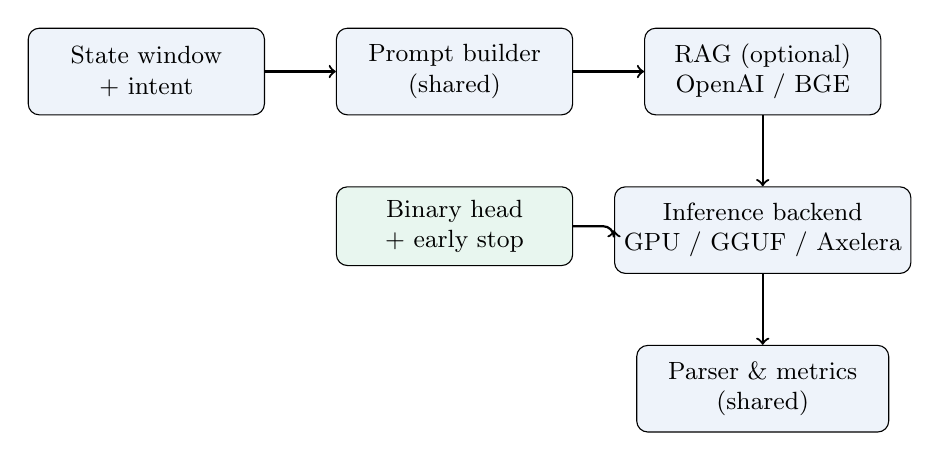
\begin{tikzpicture}[node distance=9mm, every node/.style={font=\small}, rounded corners]
    \node[draw, fill=TableHeader, align=center, minimum width=3.0cm, minimum height=1.1cm] (data) {State window\\+ intent};
    \node[draw, fill=TableHeader, right=of data, align=center, minimum width=3.0cm, minimum height=1.1cm] (prompt) {Prompt builder\\(shared)};
    \node[draw, fill=TableHeader, right=of prompt, align=center, minimum width=3.0cm, minimum height=1.1cm] (rag) {RAG (optional)\\OpenAI / BGE};

    \node[draw, fill=TableHeader, below=of rag, align=center, minimum width=3.2cm, minimum height=1.1cm] (backend) {Inference backend\\GPU / GGUF / Axelera};
    \node[draw, fill=TableHeader, below=of backend, align=center, minimum width=3.2cm, minimum height=1.1cm] (parse) {Parser \& metrics\\(shared)};

    \node[draw, fill=TableGood, below=of prompt, align=center, minimum width=3.0cm, minimum height=1.0cm] (binary) {Binary head\\+ early stop};

    \draw[->, thick] (data) -- (prompt);
    \draw[->, thick] (prompt) -- (rag);
    \draw[->, thick] (rag) -- (backend);
    \draw[->, thick] (backend) -- (parse);
    \draw[->, thick] (binary) -| (backend.west);
  \end{tikzpicture}
\end{frame}

\begin{frame}{Metrics}
  \begin{itemize}
    \item \metric{Structure-followed rate}: output matches schema (parseable).
    \item \metric{Average accuracy}: accuracy over all samples (malformed = incorrect).
    \item \metric{Parsed accuracy}: accuracy over parseable samples only.
    \item \metric{Token statistics}: prompt / RAG hint / output length (proxy for latency/energy).
  \end{itemize}
  \vspace{0.5em}
  \small
  In tables: accuracy shown as \texttt{avg | parsed}. Lower tokens are better.
\end{frame}

\begin{frame}{RAG on GPU: on-board BGE vs cloud OpenAI embeddings}
  \small
  \setlength{\tabcolsep}{4pt}
  \begin{tabularx}{\textwidth}{l l c c c}
    \toprule
    \textbf{Model} & \textbf{RAG} & {\textbf{Struct (\%)}} & {\textbf{Parsed acc (\%)}} & {\textbf{Out tok}} \\
    \midrule
    Phi-3 (3.8B) & none   & 99.18 & 72.39 & 114 \\
    \rowcolor{TableHeader}
    Phi-3 (3.8B) & OpenAI & 100.00 & \cellcolor{TableGood}\textbf{79.31} & 150 \\
    Phi-3 (3.8B) & BGE    & 100.00 & 77.86 & 160 \\
    \addlinespace
    Llama-3.2 (3.2B) & none & 98.22 & 72.10 & 120 \\
    \rowcolor{TableHeader}
    Llama-3.2 (3.2B) & BGE  & \cellcolor{TableWarn}86.42 & \cellcolor{TableGood}\textbf{80.58} & \cellcolor{TableWarn}227 \\
    \addlinespace
    Qwen2.5 (7.6B) & none & 100.00 & 81.35 & 109 \\
    \rowcolor{TableHeader}
    Qwen2.5 (7.6B) & BGE  & 100.00 & \cellcolor{TableGood}\textbf{86.55} & 124 \\
    \bottomrule
  \end{tabularx}

  \vspace{0.6em}
  \footnotesize
  Takeaway: BGE often matches the cloud retriever, but some backbones trade parsed gains for lower structure or higher verbosity.
\end{frame}

\begin{frame}{Binary decision head + early stopping (GPU)}
  \small
  \setlength{\tabcolsep}{4pt}
  \begin{tabularx}{\textwidth}{l l c c c c}
    \toprule
    \textbf{Model} & \textbf{Mode} & {\textbf{Struct (\%)}} & {\textbf{Parsed acc (\%)}} & {\textbf{Out tok}} & {\textbf{$\times$ tok}} \\
    \midrule
    Phi-3 (3.8B) & explanatory & 99.18 & 72.39 & 114 & 1 \\
    \rowcolor{TableHeader}
    Phi-3 (3.8B) & binary      & 100.00 & 70.88 & \cellcolor{TableGood}\textbf{7} & \cellcolor{TableGood}\textbf{16.3} \\
    \addlinespace
    Qwen2.5 (7.6B) & explanatory & 100.00 & 81.35 & 109 & 1 \\
    \rowcolor{TableHeader}
    Qwen2.5 (7.6B) & binary      & 100.00 & 81.47 & \cellcolor{TableGood}\textbf{7} & \cellcolor{TableGood}\textbf{15.6} \\
    \bottomrule
  \end{tabularx}

  \vspace{0.6em}
  \footnotesize
  Takeaway: for compliant backbones, early stopping cuts output tokens by $>10\times$ with small accuracy impact.
\end{frame}

\begin{frame}{GGUF quantization (Q4.M, \texttt{llama.cpp})}
  \small
  \setlength{\tabcolsep}{4pt}
  \begin{tabularx}{\textwidth}{l l l c c c}
    \toprule
    \textbf{Model} & \textbf{RAG} & \textbf{Device} & {\textbf{Struct (\%)}} & {\textbf{Parsed acc (\%)}} & {\textbf{Out tok}} \\
    \midrule
    Phi-3 (3.8B) & BGE  & GPU FP16  & 100.00 & \cellcolor{TableGood}\textbf{77.86} & 160 \\
    \rowcolor{TableHeader}
    Phi-3 (3.8B) & BGE  & GGUF Q4.M & 99.81 & 72.06 & \cellcolor{TableGood}\textbf{63} \\
    \addlinespace
    Llama-3.2 (3.2B) & none & GPU FP16  & 98.22 & \cellcolor{TableGood}\textbf{72.10} & 120 \\
    \rowcolor{TableHeader}
    Llama-3.2 (3.2B) & none & GGUF Q4.M & 99.49 & 66.78 & 185 \\
    \bottomrule
  \end{tabularx}

  \vspace{0.6em}
  \footnotesize
  Takeaway: Q4.M keeps structure high but can shift accuracy/verbosity depending on backbone and prompt.
\end{frame}

\begin{frame}{Axelera Metis (INT8): structure vs decision quality}
  \small
  \setlength{\tabcolsep}{4pt}
  \begin{tabularx}{\textwidth}{l l l c c c}
    \toprule
    \textbf{Model} & \textbf{RAG} & \textbf{Mode} & {\textbf{Struct (\%)}} & {\textbf{Avg acc (\%)}} & {\textbf{Out tok}} \\
    \midrule
    Phi-3 (3.8B) & none & GPU FP16 (exp.)    & 99.18 & \cellcolor{TableGood}\textbf{71.83} & 114 \\
    \rowcolor{TableHeader}
    Phi-3 (3.8B) & none & Axelera INT8 (exp.) & 97.02 & 55.84 & \cellcolor{TableWarn}223 \\
    Phi-3 (3.8B) & none & Axelera INT8 (bin.) & 98.41 & 66.12 & \cellcolor{TableGood}\textbf{9} \\
    \addlinespace
    Llama-3.2 (3.2B) & BGE & GPU FP16 (exp.)    & \cellcolor{TableWarn}86.42 & \cellcolor{TableGood}\textbf{69.54} & \cellcolor{TableWarn}227 \\
    \rowcolor{TableHeader}
    Llama-3.2 (3.2B) & BGE & Axelera INT8 (exp.) & \cellcolor{TableBad}49.62 & 34.33 & 188 \\
    \bottomrule
  \end{tabularx}

  \vspace{0.6em}
  \footnotesize
  Takeaway: INT8 compilation can preserve parseability yet degrade decision accuracy, pointing to quantization/compiler sensitivity.
\end{frame}

\begin{frame}{SFT improves structure and reduces verbosity (Qwen2.5)}
  \small
  \setlength{\tabcolsep}{4pt}
  \begin{tabularx}{\textwidth}{l l c c c}
    \toprule
    \textbf{Model} & \textbf{Mode} & {\textbf{Struct (\%)}} & {\textbf{Avg acc (\%)}} & {\textbf{Out tok}} \\
    \midrule
    Qwen2.5 7.6B & base (exp.) & 100.00 & 81.35 & 109 \\
    \rowcolor{TableHeader}
    Qwen2.5 7.6B & SFT (exp.)  & 100.00 & \cellcolor{TableGood}\textbf{85.28} & \cellcolor{TableGood}\textbf{71} \\
    Qwen2.5 7.6B & SFT (bin.)  & 100.00 & \cellcolor{TableGood}\textbf{85.72} & \cellcolor{TableGood}\textbf{7} \\
    \bottomrule
  \end{tabularx}

  \vspace{0.6em}
  \footnotesize
  Takeaway: SFT yields near-perfect formatting and shorter outputs while keeping strong decision accuracy.
\end{frame}

\begin{frame}{Takeaways \& next steps}
  \begin{itemize}
    \item On-board RAG (BGE) can recover much of cloud RAG’s benefit while remaining self-contained.
    \item Binary decision heads + early stopping are a high-leverage knob for embedded latency/energy.
    \item GGUF quantization is a practical path to smaller footprints with moderate accuracy shifts.
    \item Axelera INT8 shows strong structure but inconsistent decision quality: vendor quantization/compiler pipeline matters.
    \item Next: finish power profiling (energy/decision), and tune INT8 compilation for decision robustness.
  \end{itemize}
  \vfill
  \footnotesize
  Repository: \texttt{github.com/fgarciacardenas/RISCVxLLMxRobot}
\end{frame}

\end{document}
